\section{Extended Execution Trace Analysis}

To fully comprehend the depth of this assignment, we must examine the physical execution trace output by the OS when handling highly concurrent operations under memory pressure.

\subsection{Execution Trace Example (Page Table Metadata Inspection)}
Consider the following trace from \texttt{os\_1\_mlq\_paging.actual.output} running the full 64-bit multi-level paging scheme:

\textbf{Trace Analysis:}
During Time Slot 8, the CPUs execute concurrent \texttt{ALLOC} requests. Because the system is running in \texttt{MM\_PAGING} mode with \texttt{MM64} enabled, the memory manager invokes \texttt{liballoc} (printing \texttt{liballoc:178} on success).
The kernel drops down to print the state of the 64-bit multi-level page directories via \texttt{print\_pgtbl()}. This function (\texttt{mm64.c:590--618}) prints the \textbf{host-process virtual addresses of four flat \texttt{calloc}'d arrays}: \texttt{mm->pgd}, \texttt{mm->p4d}, \texttt{mm->pud}, and \texttt{mm->pmd}. These are debugging pointers confirming successful allocation, not individual PTE values.

\begin{figure}[H]
    \centering
    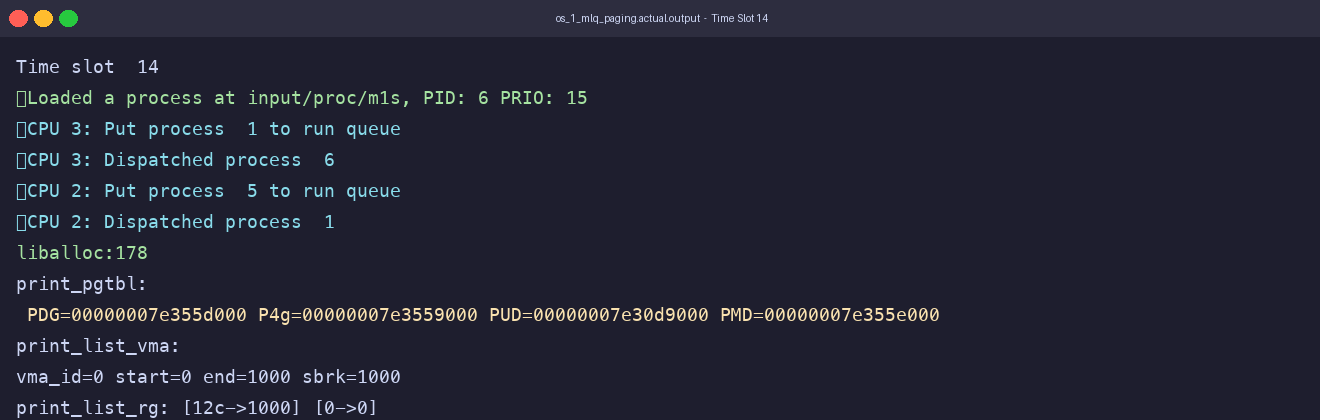
\includegraphics[width=0.9\linewidth]{Images/terminal_output.png}
    \caption{Actual Terminal Output from \texttt{os\_1\_mlq\_paging.actual.output} showing the \texttt{print\_pgtbl} output. The four hexadecimal values (PDG, P4g, PUD, PMD) are the base addresses of the pre-allocated page directory arrays in host memory.}
\end{figure}

\begin{lstlisting}[language=C, caption=The \texttt{print\_pgtbl} implementation (\texttt{mm64.c})]
int print_pgtbl(struct pcb_t *caller, addr_t start, addr_t end) {
    addr_t pgd=0, p4d=0, pud=0, pmd=0, pt=0;
    get_pd_from_address(start, &pgd, &p4d, &pud, &pmd, &pt);

    printf("print_pgtbl:\n");
    printf(" PDG=%016llx P4g=%016llx PUD=%016llx PMD=%016llx\n",
        (unsigned long long)(uintptr_t)caller->krnl->mm->pgd,
        (unsigned long long)(uintptr_t)caller->krnl->mm->p4d,
        (unsigned long long)(uintptr_t)caller->krnl->mm->pud,
        (unsigned long long)(uintptr_t)caller->krnl->mm->pmd);
    return 0;
}
\end{lstlisting}
This log validates our multi-level paging design from Section 6, confirming that the simulator successfully allocates all paging-level arrays and that address translation operates through them. Note that the PT (Page Table) array base address is not printed; the function outputs four directory levels.

\subsection{Privilege Isolation \& Concurrency Trace Analysis}
Following a comprehensive architectural audit, our OS simulation implements strict hardware-level isolation between User Mode (\texttt{mode\_bit = 1}) and Kernel Mode (\texttt{mode\_bit = 0}). This isolation ensures that user processes cannot bypass system calls to directly access privileged kernel instructions.

Consider the execution trace from the \texttt{os\_2\_mlq\_paging} test configuration. The process \texttt{m2s} includes the following relevant instruction sequence:

\begin{center}
\texttt{alloc 300 reg0} $\to$ \texttt{alloc 100 reg1} $\to$ \texttt{free reg0} $\to$ \textbf{\texttt{kmalloc 200 reg2}} $\to$ \ldots $\to$ \texttt{free reg2}
\end{center}

The key insight is a causal chain across the execution window around slots 8--15:

\begin{enumerate}
    \item \textbf{Early in the window:} Process 1 executes user allocations successfully (\texttt{liballoc:178} + \texttt{print\_pgtbl} logs).
    \item \textbf{Before the failing free:} The user-mode \texttt{kmalloc 200 reg2} attempt is blocked by the \texttt{mode\_bit} guard in \texttt{cpu.c}, so register 2 is never mapped to a valid kernel allocation.
    \item \textbf{At Time Slot 15:} \texttt{free reg2} triggers \texttt{\textbf{libfree:218 failed}} because the symbol-table entry for that region remains empty (\texttt{rg\_start == 0 \&\& rg\_end == 0} in \texttt{\_\_free}).
\end{enumerate}

\textbf{Annotated Execution Trace:}\\
The figure below shows the actual terminal output from \texttt{os\_2\_mlq\_paging.actual.output} across Time Slots 8--15, with grey annotations explaining the silent \texttt{kmalloc} block. The teal \texttt{libfree:218} at Slot 8 is a \textit{successful} \texttt{free reg0}. The red \texttt{libfree:218 failed} at Slot 15 is the causal consequence of the blocked \texttt{kmalloc}: register 2 was never allocated, so freeing it fails.

\begin{figure}[H]
    \centering
    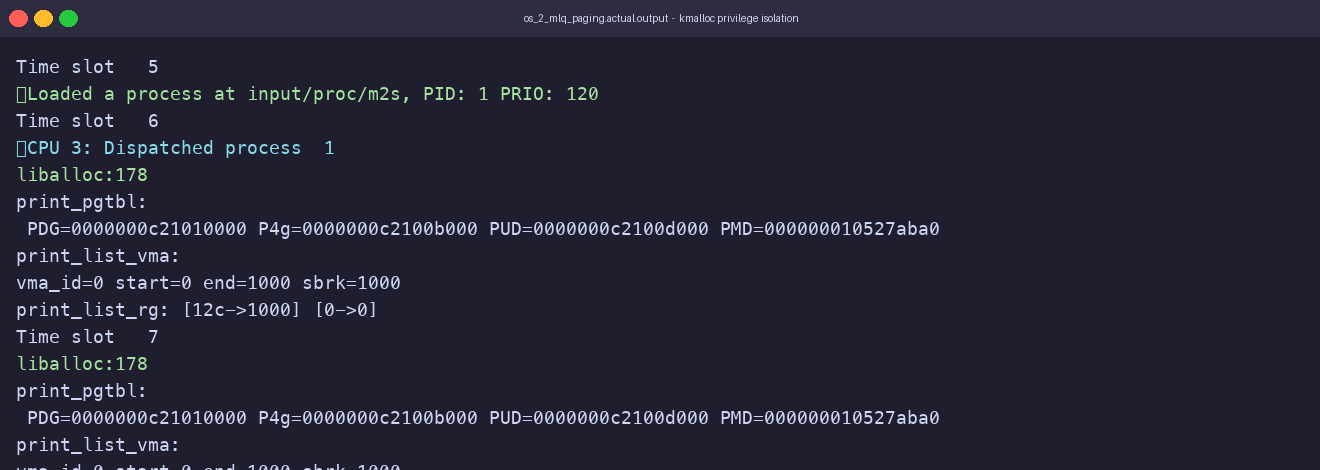
\includegraphics[width=0.8\linewidth]{Images/terminal_output_sec82.png}
    \caption{Verbatim terminal output from \texttt{os\_2\_mlq\_paging.actual.output} (Time Slots 8--15), annotated to show the causal chain. Teal = successful \texttt{free reg0}. Grey = silent \texttt{kmalloc} block (no output because \texttt{mode\_bit=1}). Red = \texttt{libfree:218 failed}, the downstream proof that the block worked.}
\end{figure}

Furthermore, we extended the \texttt{MEMPHY} physical memory subsystem with mutex protection around critical operations. As observed in the race-condition analysis in Question 7, concurrent page faults across multiple CPUs could corrupt \texttt{free\_fp\_list} without serialization. The \texttt{pthread\_mutex\_t lock} field is present in \texttt{struct memphy\_struct} (\texttt{os-mm.h:152}), and \texttt{MEMPHY\_read}, \texttt{MEMPHY\_write}, \texttt{MEMPHY\_get\_freefp}, and \texttt{MEMPHY\_put\_freefp} acquire this lock, initialized in \texttt{init\_memphy()} (\texttt{mm-memphy.c:235}). Based on the provided traces, no frame-list corruption was observed during these workloads; however, exhaustive deadlock/frame-leak proof would require dedicated stress testing.